\documentclass[a4paper, 12pt, twoside, titlepage, french]{beamer}
\usetheme{Warsaw}
\usepackage{color}
\usepackage{listings}
\usepackage{physics, amsmath,amsthm,verbatim,amssymb,amsfonts,amscd, graphicx, amscd, yfonts, mathrsfs}
\usepackage[utf8]{inputenc}
%\usepackage[hmargin={3.5cm,3.5cm},top=4cm,bottom=4cm]{geometry} %problem...
\graphicspath{ {../images/} }
\usepackage{physics}
\RequirePackage[utf8]{inputenc}
\RequirePackage[T1]{fontenc}
\RequirePackage{babel}

\RequirePackage{cleveref}
\newtheorem{theoreme}{Théorème}
%%%%%%%%%%%%%%%%%%%%%%%%%%%%
\lstset{ %
  backgroundcolor=\color{white},   % choose the background color; you must add \usepackage{color} or \usepackage{xcolor}
  basicstyle=\small,        % the size of the fonts that are used for the code
  commentstyle=\color{blue},    % comment style
  extendedchars=true,              % lets you use non-ASCII characters; for 8-bits encodings only, does not work with UTF-8
  keepspaces=true,                 % keeps spaces in text, useful for keeping indentation of code (possibly needs columns=flexible)
  keywordstyle=\color{red},       % keyword style
  language=Fortran,                 % the language of the code
  rulecolor=\color{black},         % if not set, the frame-color may be changed on line-breaks within not-black text (e.g. comments (green here))
  showspaces=false,                % show spaces everywhere adding particular underscores; it overrides 'showstringspaces'
  showstringspaces=false,          % underline spaces within strings only
  showtabs=false,                  % show tabs within strings adding particular underscores
  stringstyle=\color{green},     % string literal style
  tabsize=2,	                   % sets default tabsize to 2 spaces
  frame=single
}



%%%%%%%%%%%%%%%%%%%%%%%%%%%%%%%%%%%%%%%%%%%%%%%%%%%%%%%%%%%%%%%%%%%%%%%%
\title{Propriétés spectroscopique}
\author{En-Hung CHAO, Honghao LI}
\institute{École Polytechnique}
\date{\today}
%%%%%%%%%%%%%%%%%%%%%%%%%%%%%%%%%%%%%%%%%%%%%%%%%%%%%%%%%%%%%%%%%%%%%%%%
%%%%%%%%%%%%%%%%%%%%%%%%%%%%%%%%%%%%%%%%%%%%%%%%%%%%%%%%%%%%%%%%%%%%%%%%
\begin{document}


\begin{frame}
\titlepage
\end{frame}
%%%%%%%%%%%%%%%%%%%%%%%%%%%%%%%%%%%%%%%
%%%%%%%%%%%%%%%%%%%%%%%%%%%%%%%%%
\begin{frame}
\frametitle{Plan de présentation}
\framesubtitle{}
\begin{enumerate}
\item Introduction
\item Études de l'état fondamental
\item Études des états excités
\item Conclusion 
\end{enumerate}
\end{frame}
%%%%%%%%%%%%%%%%%%%%%%%%%%%%%%%%%%%%%%%

\begin{frame}
\frametitle{Introduction}
\framesubtitle{}
\begin{itemize}
\item Les études spectroscopiques
\item Les calculs $ab initio$
\item Le choix du matériau: l'oxalate de calcium
\item Les calculs numériques
\end{itemize}
\end{frame}
\newpage
%%%%%%%%%%%%%%%%%%%%%%%%%%%%%%%%%%%%%%%%%%%%%%%%%%%%%%%%%%%%%

\begin{frame}
\frametitle{Études de l'état fondamental}
\framesubtitle{Structure de l'oxalate de calcium}
La cellule élémentaire de l'oxalate de calcium ($CaC_2O_4$) contient 28 atomes et est de structure monoclinique.
\begin{figure}[!h]
  \centering
  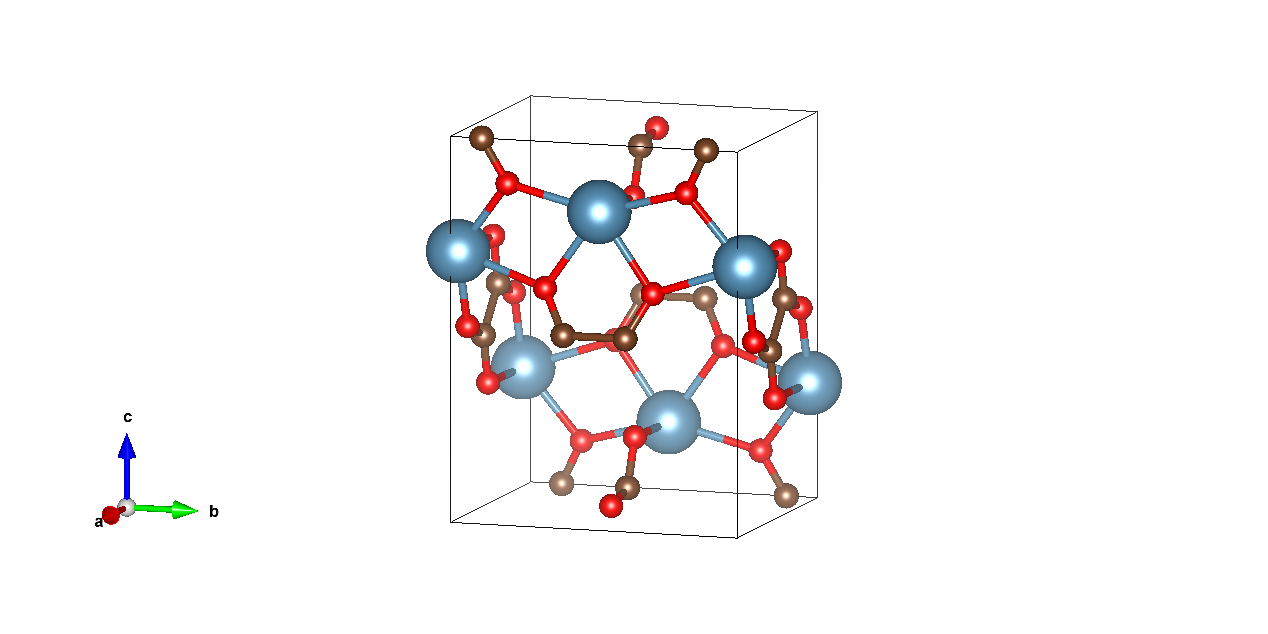
\includegraphics[height=0.4\textheight]{co_structure}
  \caption{La cellule élémentaire de l'oxalate de calcium avec $Ca$ en bleu, $O$ en rouge et $C$ en marron.}\label{BrillouinZone}
\end{figure}
\end{frame}
\newpage

%%%%%%%%%%%%%%%%%%%%%%%%%%%%%%%%%%%%%%%%%%%%5555
\begin{frame}
\frametitle{Études de l'état fondamental}
\framesubtitle{DFT}
\begin{theoreme}[Hohnenberg-Kohn]
  L'espérance d'un observable dans l'état fondamental est une fonctionnelle unique
  de la densité d'électrons.
\end{theoreme}

\begin{theoreme}[Kohn-Sham]
  Pour tout système qui contient des termes d'interactions entre électrons,
  il existe un système auxiliaire non-interagissant ayant la même densité d'électrons.
\end{theoreme}

\textbf{Conclusion} la résolution d'un système à plusieurs corps se réduit à la recherche de la fonction de la densité d'un système d'électrons non-interagissant.
\end{frame}
\newpage
%%%%%%%%%%%%%%%%%%%%%%%%%%%%%%%%%%%%%%%%%%%%%%
\begin{frame}
\frametitle{Études de l'état fondamental}
\framesubtitle{Théorie de la fonctionnelle de la densité, DFT en anglais}
Le nouveau système d'équations à considérer

\begin{equation}
  (-\frac{1}{2}\nabla_i + V_{tot}[n](\textbf{r}))\phi_i(\textbf{r}) = \epsilon_i\phi_i(\textbf{r})
\end{equation}
avec

\begin{equation}
  V_{tot}(\textbf{r}) = \underbrace{V_{ext}(r)}_\text{ions}
  + \underbrace{\int d \textbf{r}' \frac{n(\textbf{r}')}{|\textbf{r} - \textbf{r}'|}}_\text{potentiel de Hatree}
  + \underbrace{V_{xc}([n], \textbf{r})}_\text{échange-corrélation}
\end{equation}

\textbf{Remarque} un terme d'échange-corrélation apparaît $\Longrightarrow$ approximations nécesitées (avec l'approximation des gradients généralisés, GGA en anglais)
\end{frame}
\newpage
%%%%%%%%%%%%%%%%%%%%%%%%%%%%%%%%%%%%%%%%%%%%%%%%%%%%%%%%%%%%%
\begin{frame}
\frametitle{Études de l'état fondamental}
\framesubtitle{Calculs numériques}
\begin{itemize}
\item Réalisé avec le code d'\textit{Abinit}.
\item Fonctionnement:
Théorème de Bloch
\begin{equation*}
  \phi_{n,\textbf{k}_i}
  = \frac{1}{\sqrt{\Omega_{maille}}}e^{i\textbf{k}_i\cdot\textbf{r}}\sum_{\textbf{G}} c_{n,\textbf{k}_i}(\textbf{G})e^{i\textbf{G}\cdot\textbf{r}}
  = e^{i\textbf{k}_i\cdot\textbf{r}} u_{n,\textbf{k}_i}(\textbf{r})
\end{equation*}
\item Réduction de la dimension de la base d'ondes planes en définissant une énergie de seuil $E_{cut}$:
   	\begin{equation}
      \frac{1}{2}|\textbf{k}+\textbf{G}|^2 \leq E_{cut}
	\end{equation}    
    avec relation entre les ondes planes dans la base et $E_{cut}$:
    \begin{equation}
      N_{op}\propto E_{cut}^{\frac{3}{2}}.
    \end{equation}
 

\end{itemize}

\end{frame}

%%%%%%%%%%%%%%%%%%%%%%%%%%%%%%%%%%%%%%%%%%%%%%%%
\begin{frame}
\frametitle{Études de l'état fondamental}
\framesubtitle{Convergence en énergie de seuil du système}
\begin{figure}[!h]
    \centering
    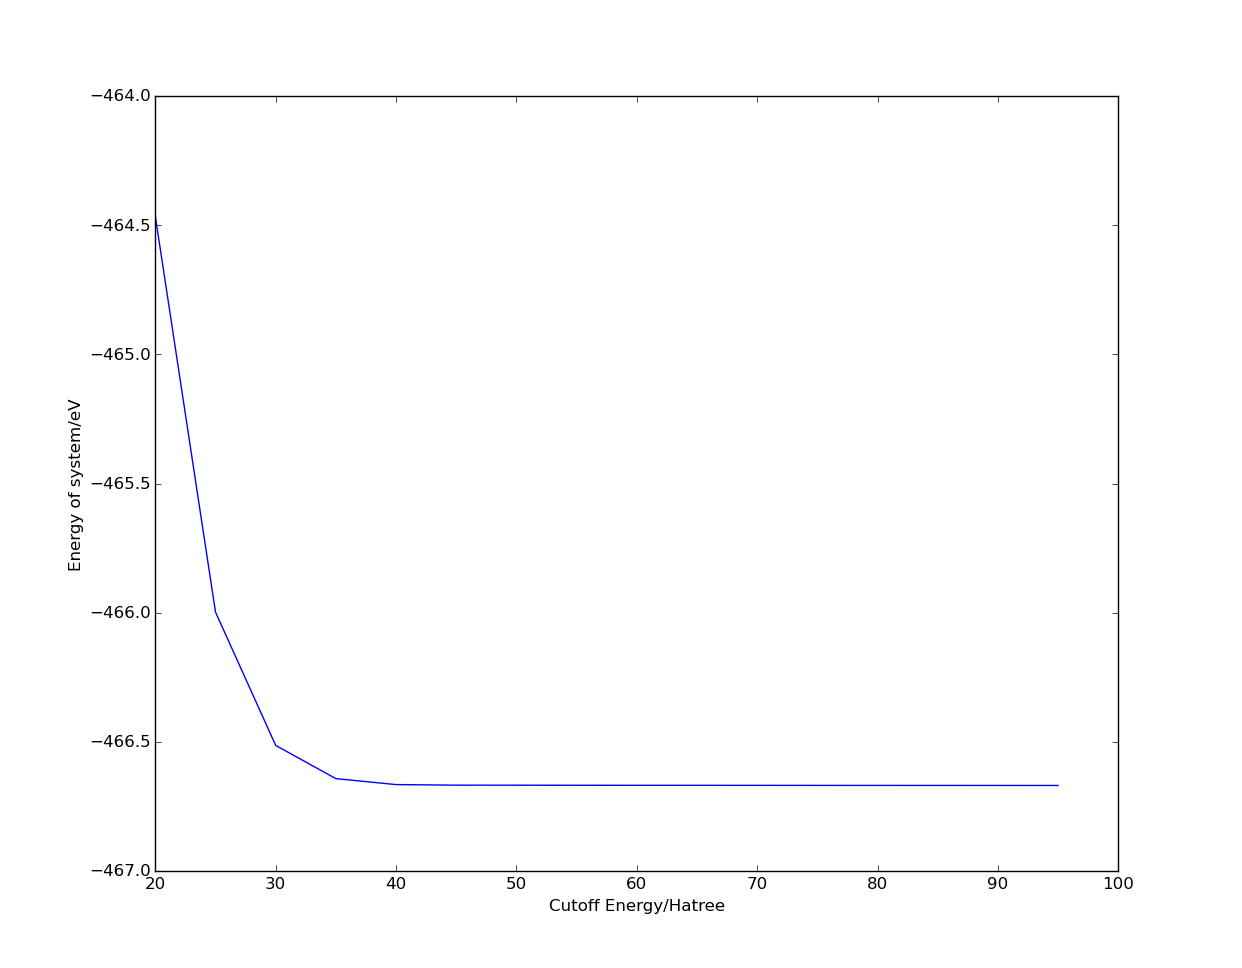
\includegraphics[width=8cm]{E_cut}
    \caption{L'énergie totale du système (en eV) en fonction de l'énergie de seuil (en Hatree).}\label{fig-Ecut}
\end{figure}
\end{frame}

%%%%%%%%%%%%%%%%%%%%%%%%%%%%%%%%%%%%%%%%%%%%%%%%
\begin{frame}
\frametitle{Études de l'état fondamental}
\framesubtitle{Convergence de l'échantillonnage}
\begin{itemize}
\item Calul discrétisé dans l'espace de Fourier $\Longrightarrow$ échantillonnage de la première zone de Brillouin
\item Choix d'échantillonnage pertinents (respectant les symétries du problème)

\end{itemize}
\begin{table}[ht]
  \caption{Énergie totale du système en fonction du nombre de points-$\textbf{k}$}
  \centering
  \begin{tabular}{c c}
    \hline
    Nombre de points-$\textbf{k}$  &  $E_{tot}$ à la convergence (Hatree)
    \\
    \hline
    16    &  -466.66501448840
    \\
    28    &  -466.66501224916
    \\
    40    &  -466.66501098806
    \\
    \hline
  \end{tabular}
\end{table}

\end{frame}

%%%%%%%%%%%%%%%%%%%%%%%%%%%%%%%%%%%%%%%%%%%%%%%%
\begin{frame}
\frametitle{Études des états excités}
\framesubtitle{TDDFT}
\begin{itemize}
\item Théorie de la fonctionelle de la densité dépendante du temps
\item Absorption et spectre de pertes en énergie (EELS)
\begin{equation}
  \textrm{Abs} = \mathcal{I}\{\epsilon(\omega, \textbf{q})\},
  \quad
  \textrm{EELS} = -\mathcal{I}\{\epsilon(\omega, \textbf{q})^{-1}\}.
\end{equation}

\begin{figure}[!h]
  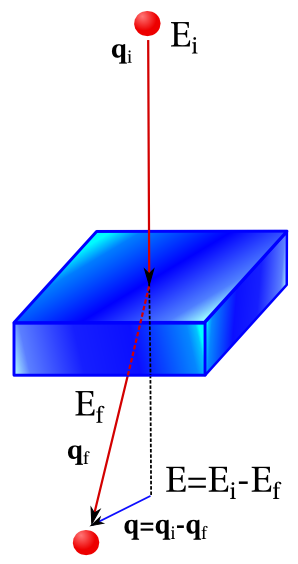
\includegraphics[width=0.2\textwidth]{eels}
  \caption{Dispersion et moment transféré}
\end{figure}
\end{itemize}
\end{frame}

%%%%%%%%%%%%%%%%%%%%%%%%%%%%%%%%%%%%%%%%%%%%%%%%
\begin{frame}
\frametitle{Études de l'état fondamental}
\framesubtitle{DFT}
\begin{itemize}
%TODO reformulate this
\item Relation entre la polarisabilité  et la fonction diélectrique
\begin{equation*}
  \epsilon^{-1} = 1+ v\chi.
\end{equation*}
\item Relation entre $\chi$ et $\chi^0$
\begin{equation*}
\chi = \chi^0 ( 1 + (v+f_{\textrm{xc}})\chi)
\end{equation*}
$\Longrightarrow$ terme d'échange-corrélation à approximer.
\end{itemize}
 
\end{frame}

%%%%%%%%%%%%%%%%%%%%%%%%%%%%%%%%%%%%%%%%%%%%%%%%
%\newpage
%\addcontentsline{toc}{section}{Bibliographie}
%\begin{thebibliography}{99}

%\bibitem{Unity}

%\end{thebibliography}

\end{document}
